\section{R2U2 Software (Python)(Requires python 3.X)}
The current python version only supports offline test. Python R2U2 is suitable for research purpose if you want to check how the SCQ works or the observer algorithm.
The python version code is located under the repository: \colorbox{gray!30}{r2u2/R2U2\_SW/R2U2\_PYTHON/}.
\subsection{Process Overflow}
\begin{figure}[H]
	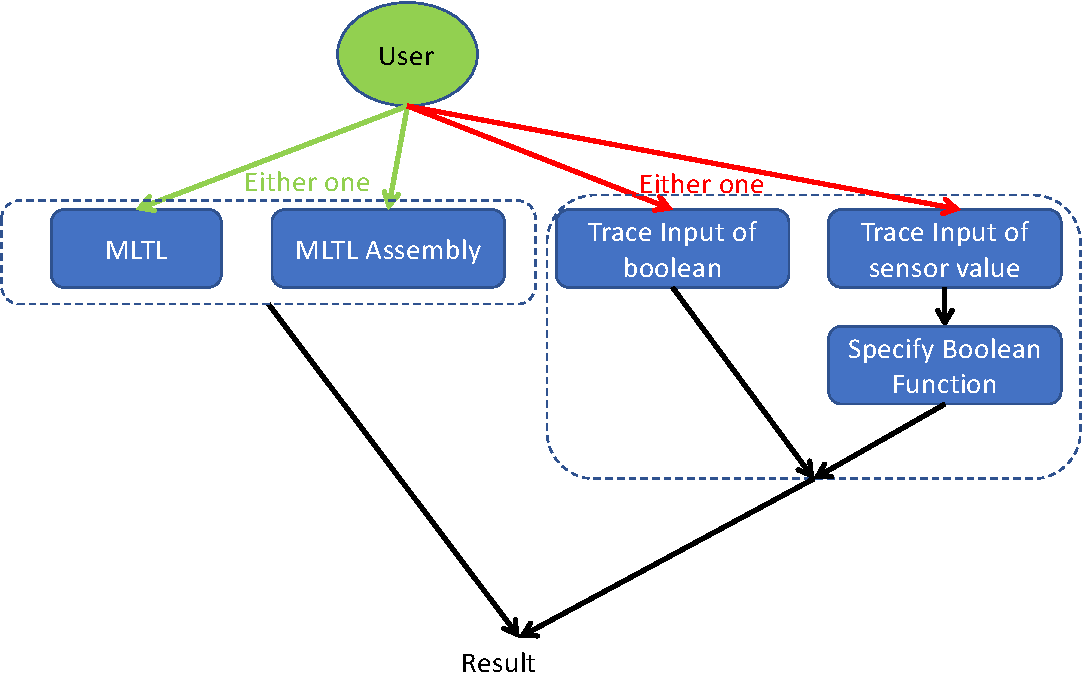
\includegraphics[scale=0.50]{fig/r2u2_python_flow.pdf}
	\caption{Deploying steps of R2U2 Python.}
	\label{fig:python_flow}
\end{figure}

User can run the R2U2 python in terminal:
\begin{lstlisting}[language=Bash]
	python MLTL_main.py -m "$(cat [A])" -s [B] -o [C]
\end{lstlisting}
\begin{tcolorbox}
A: Assembly/MLTL Input File: Assembly code in a file or MLTL formula written in a file\\
B: Signal Trace File. Refer to Section \ref{sec:python_trace_format} for detail format. \\
C: Output File. The RV result will be written into the file. If user did not specify \textbf{-o} option, the output file will be default 'untitled.txt'.
\end{tcolorbox}
Or
\begin{lstlisting}[language=Bash]
	python MLTL_main.py -m [A] -s [B] -o [C]
\end{lstlisting}
\begin{tcolorbox}
A: MLTL formula (Take care of special symbol in command line)\\
B: Signal Trace File. Refer to Section \ref{sec:python_trace_format} for detail format. \\
C: Output File. The RV result will be written into the file. If user did not specify \textbf{-o} option, the output file will be default 'untitled.txt'.
\end{tcolorbox}


\subsection{Input Trace Format and Boolean Function}
\label{sec:python_trace_format}
Table \ref{tab:python_trace} shows the input format for the trace input file.
\begin{table}[ht]
	\caption{Format and content of trace file}
	\label{tab:python_trace}
	\begin{center}
	\begin{tabular}{c|cccc|cccc}
		\hline
		Mode&\multicolumn{4}{c|}{Atomic Input Format(0/1)}&\multicolumn{4}{c}{Sensor Input Format(floating)}\\
		\cline{1-9}
		\multirow{1}{*}{Column Information}&atomic 0&atomic 1&atomic 2&\multicolumn{1}{c|}{...}&sensor 0&sensor 1&sensor 2&...\\
		\hline
		\multirow{3}{*}{trace file content}& a0 & a1 & a2 &...& altitude & velocity & temp &...\\
		& 0 & 1 & 1 &...  & 1005& 32.7 &87 \\
		& 0 & 0 & 1 &... & 1010& -1.7 &87  \\
		&...& & & ...& ...&  & \\
		\hline
	\end{tabular}
	\end{center}
	\label{tab:multicol}
	\end{table}
In the trace input file, the first row is the trace name. After the first row, each line is the data in a seperate time stamp ranging from 0. E.g., the second row is data in time stamp 0, third row is data in time stamp 1. For each column (split by either space or comma), the first column data is signal trace 0. The second column data is signal trace 1 and so on. \\
Note that 1) For atomic input format, the atomic name should be consistent with the atomic name in MLTL specification; 2) For sensor Input, the sensor name should be consistent with the boolean function in \colorbox{gray!30}{r2u2/R2U2\_SW/R2U2\_PYTHON/ACOW/Traverse.py} function \colorbox{blue!30}{s2a(self,signal\_trace)}. The atomic map in the function should be consistent with the MLTL specification. Below is the example for function \colorbox{blue!30}{s2a(self,signal\_trace)}:
\begin{lstlisting}[language=Python]
def s2a(self,signal_trace):	
	atomic_map = {}
	s2d = {signal_name:i for i,signal_name in enumerate(self.trace_name)}

	##################################################################
	# For User: map boolean function to atomic
	atomic_map['a0'] = abs(s2d['altitude'])<0.04
	atomic_map['a1'] = abs(s2d['velocity'])<0.08
	atomic_map['a2'] = s2d['temp']>0.6
	##################################################################
	return atomic_map
\end{lstlisting}

\subsection{AST Optimization}
AST optimization only works in MLTL formula input. If you want to optimize the AST, change the input argument in function \colorbox{blue!30}{formula\_input()}. The following line of code in MTL\_main.py:
\begin{lstlisting}[language=Python]
	valid_node_set = formula_input(MLTL) # optimize
	valid_node_set = formula_input(MLTL,False) # unoptimize
\end{lstlisting}

\subsection{Model Checking (not used in R2U2)}
\subsubsection{Define Automata} \label{sec:aut}
You can specify the input as the automata.
\begin{lstlisting}[language=Python]
def define_automaton():
	a = automaton()
	#sg = StateGen(3,'s','a') # call function to autogenerate state for you
	a.INITIAL_STATE = 's2'
	a.DEST_STATE = 's3'
	#a.STATE, a.DELTA = sg.gen_aut()
	a.STATE = {
	's0':{'a0':0,'a1':0},
	's1':{'a0':0,'a1':1},
	's2':{'a0':1,'a1':0},
	's3':{'a0':1,'a1':1},
	}
	a.DELTA = {
	's0': {'s0','s1','s2','s3'},
	's1': {'s0','s1','s2','s3'},
	's2': {'s0','s1','s2','s3'},
	's3': {'s0','s1','s2','s3'},
	}
	print(a)
	return a
\end{lstlisting}

\subsubsection{Run Model Checking}
The tool supports model checking for a MLTL formula given the automata. User need to define the automata with initial state \textbf{INITIAL\_STATE} and desired end state \textbf{DEST\_STATE}.
\begin{lstlisting}[language=Python]
	a = define_automaton()
	a.init()
	valid_node_set = assembly_input(MLTL)
	solution = Search(a,valid_node_set,agent='DES')
\end{lstlisting}
\clearpage
